%%% File encoding is ISO-8859-1 (also known as Latin-1)
%%% You can use special characters just like �,� and �

\chapter{Results}
\begin{figure}[H]
\begin{center}
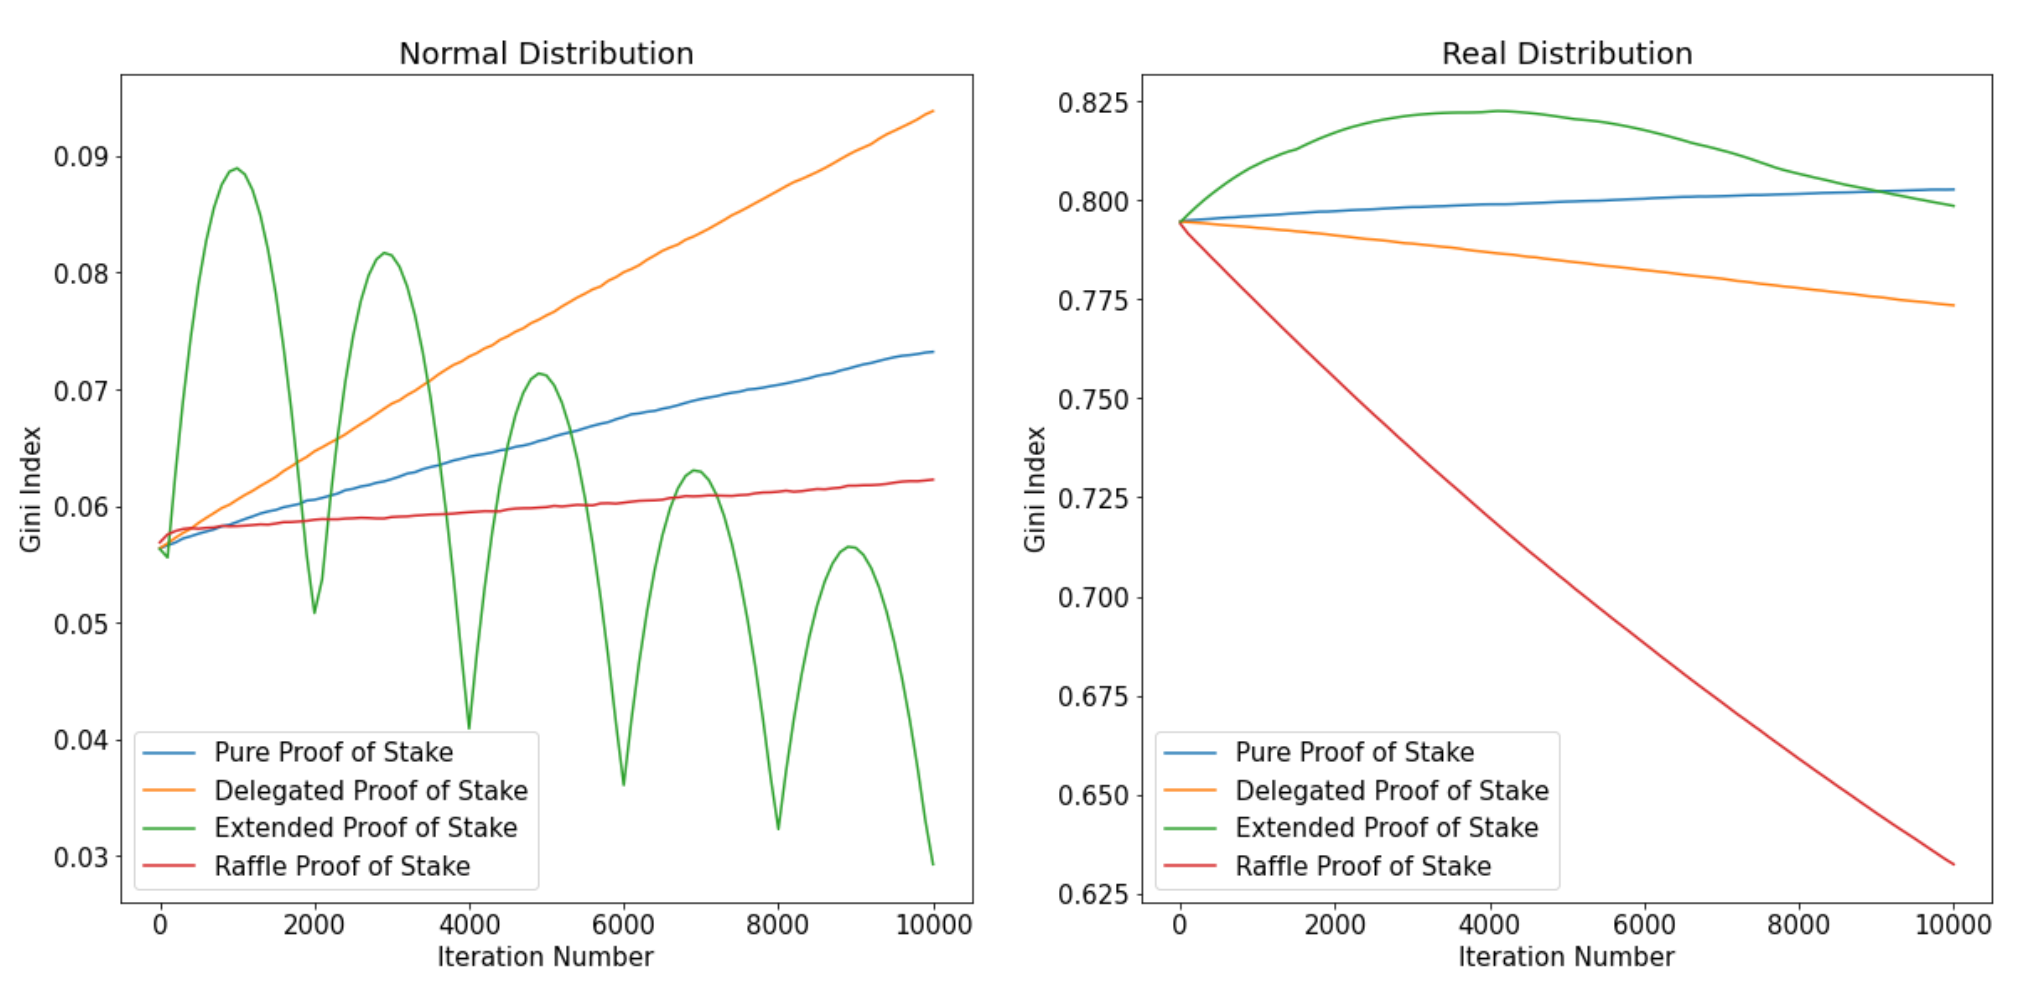
\includegraphics[width=1\textwidth]{03_Graphics/comparison}
\caption{Performance Comparison of All Protocols}
\label{fig:comp}
\end{center}
\end{figure}
\section{Pure Proof-of-Stake}
Based on our simulations with normal and real distributions of wealth, we found that P-PoS has a trend of increasing centralization over time. As described earlier, P-PoS carries out a pseudorandom selection process to determine validators of blocks, weighted by the amount of stake that the user has in the system. The more stake a user has, the more likely they are to be selected based on the factor of stake in random selection over time.
\begin{figure}[H]
\begin{center}
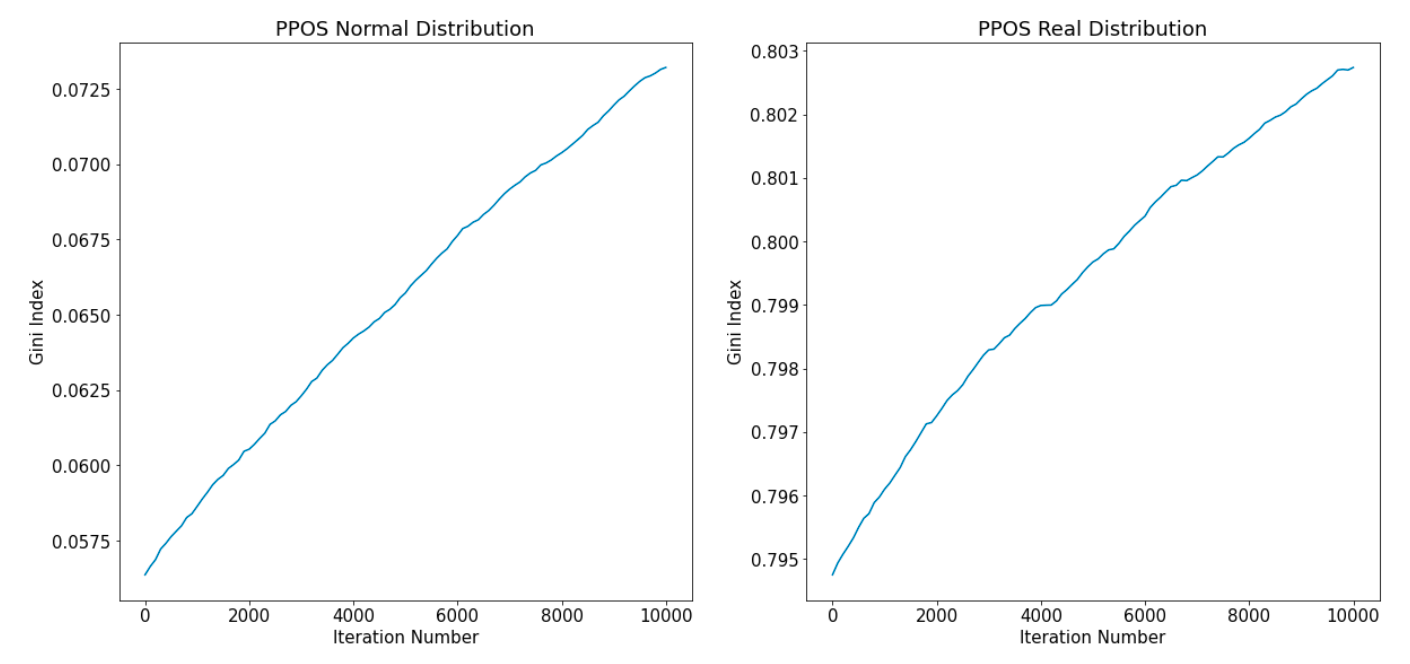
\includegraphics[width=1\textwidth]{03_Graphics/ppos_comp}
\caption{Performance of Pure Proof of Stake}
\end{center}
\end{figure}
Once a user is selected and wins the reward for verifying a block, they increase their total wealth and now have more that they can potentially stake in the system. This means as they keep winning, their probability of winning increases assuming they continue to increase the amount which they stake. In our model, we assume each user stakes their total wealth, as this presents the highest probability of them winning and there is no penalty for not being selected. As we can see in the performance graph of our model, the Gini coefficient increases linearly with the number of iterations of our simulation that are run.

\section{Delegated Proof-of-Stake}
\begin{figure}[H]
\begin{center}
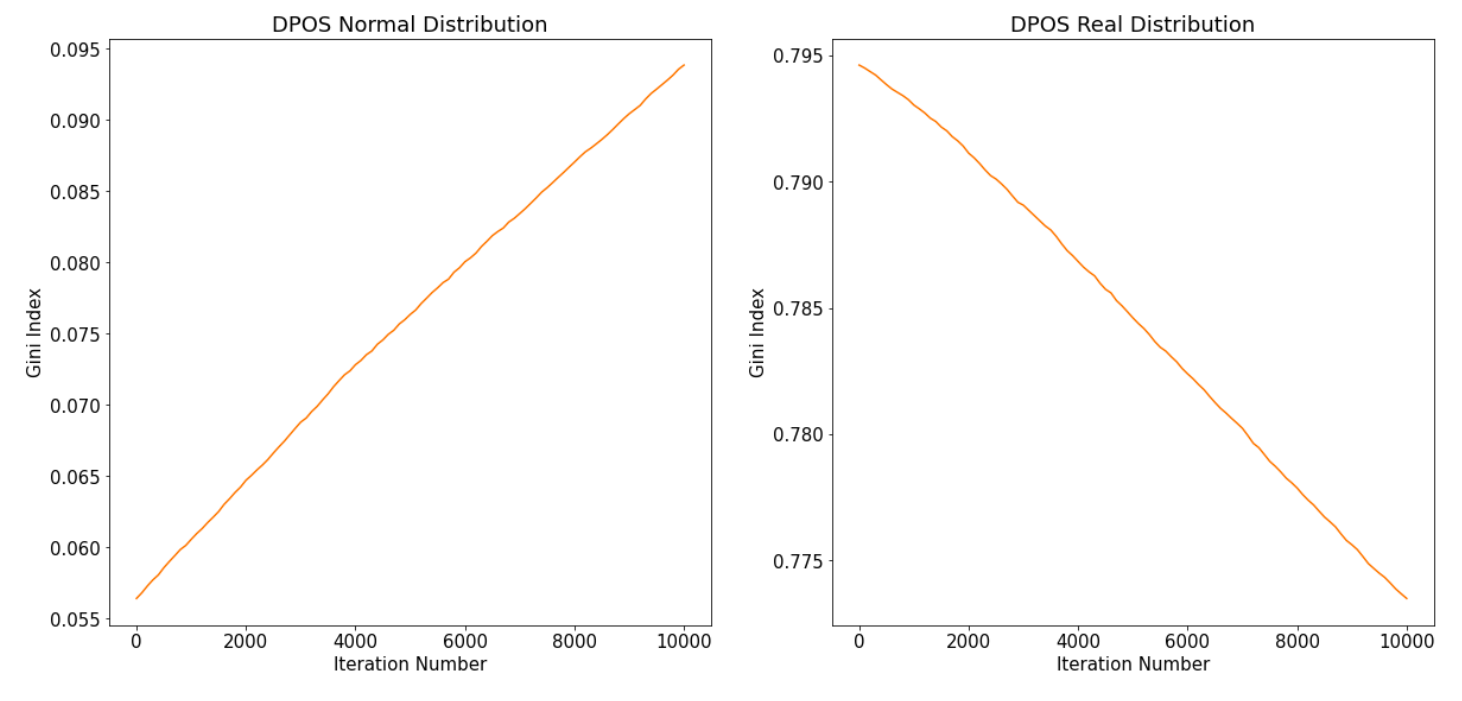
\includegraphics[width=1\textwidth]{03_Graphics/dpos_comp}
\caption{Performance of Delegated Proof of Stake}
\end{center}
\end{figure}
In a system that starts off very centralized, much like how a pre-mined coin, or a coin with reservations for early investors\slash developers, we see that delegated Proof-of-Stake performs fairly well in terms of reducing centralization. However, in a largely decentralized network, it causes rapid centralization of wealth.

The hypothesis for why the centralization shoots up rapidly in a very decentralized ecosystem is that the pool operators all rapidly increase their own wealth as they proceed to take a cut from every block mined. So their expected value from the network is higher since they are providing the service of creating and validating new blocks. However, in a highly centralized network, the trade-off between greed and popularity incentivizes the pools to compete and they end up splitting the wealth more fairly.

\section{Extended Proof-of-Stake}
For our simulation, we attempted to model this algorithm as closely as possible. To start off, we assigned each node an initial wealth and set the number of blocks validated of each node to 0. Afterwards, we created the blocks and assigned each block a random total transaction cost. After sorting the blocks in decreasing order of total transaction cost, we allowed each node to place a bid on the block they wanted to potentially validate. Assuming each node is greedy and wants to earn the most amount of coins, each node would place a bid on the highest total transaction cost block that does not exceed their total balance. In addition, the node would also commit 100\% of their remaining balance in an attempt to out-commit other nodes. We then place each node into a list of nodes associated with a given block. Finally, we run the E-PoS algorithm on each block, along with the corresponding list of potential nodes calculated from earlier.
\begin{figure}[H]
\begin{center}
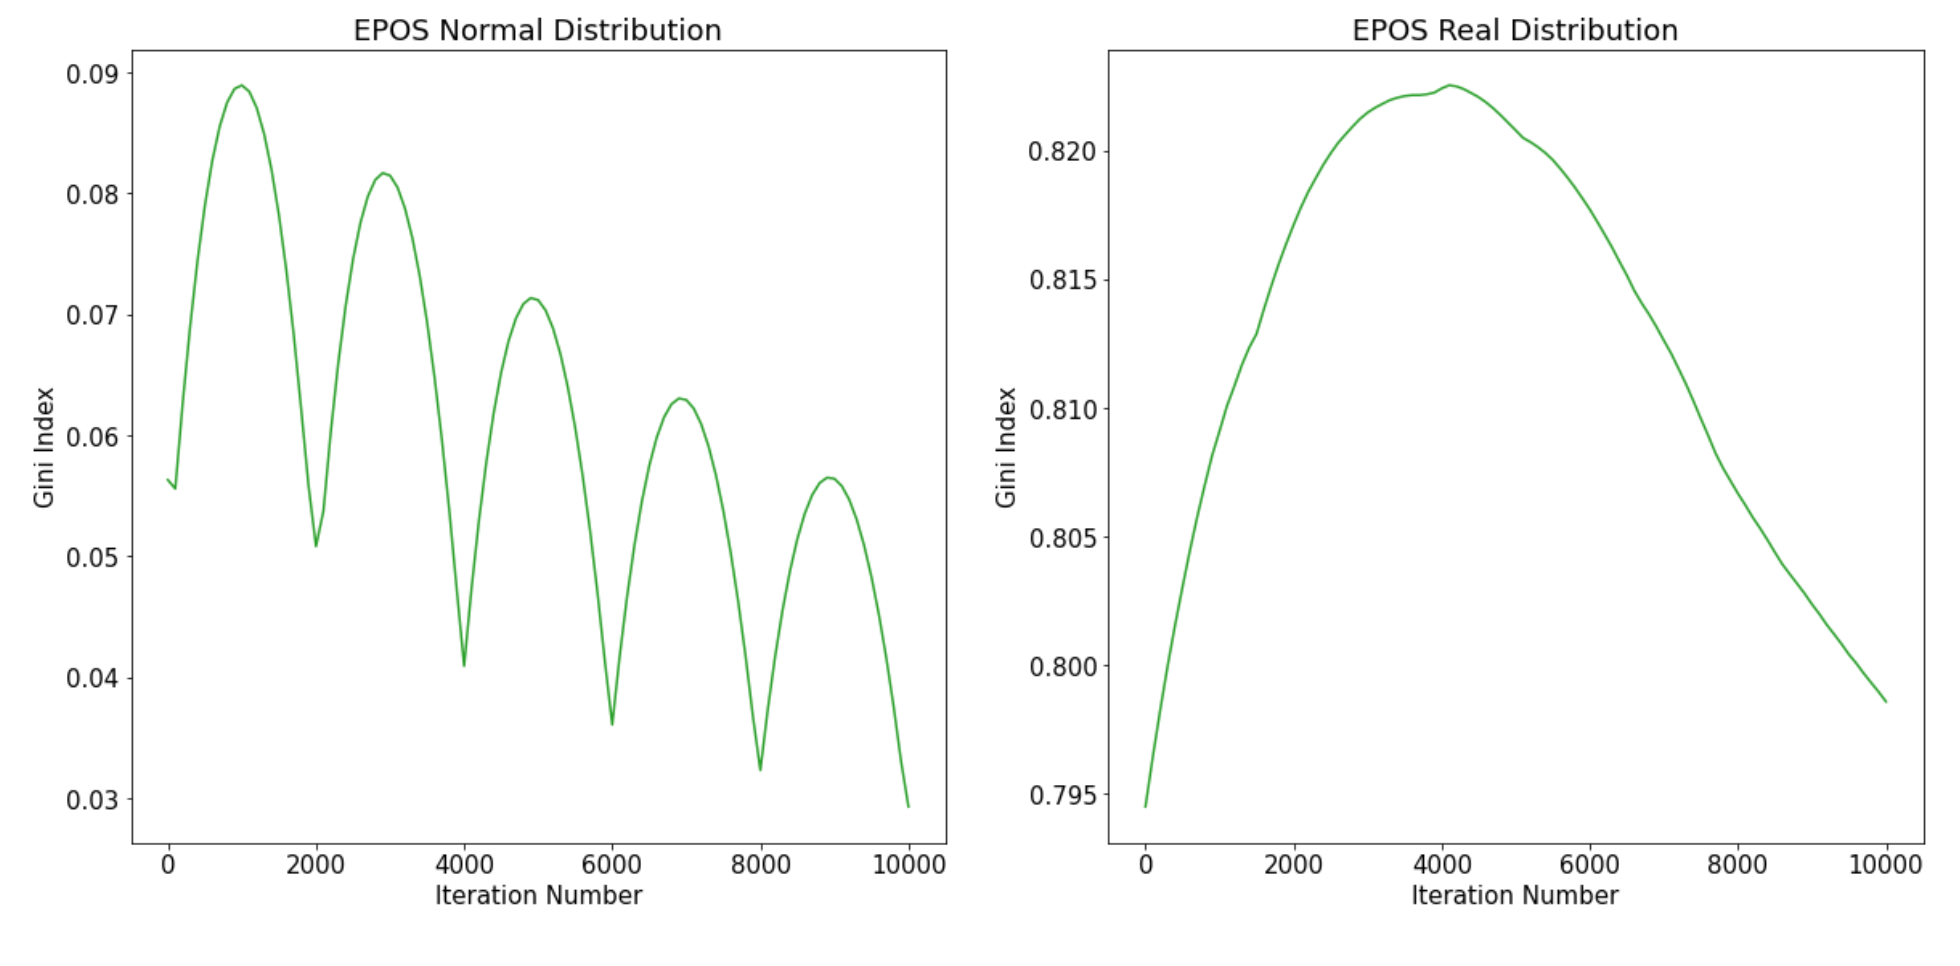
\includegraphics[width=1\textwidth]{03_Graphics/epos_comp}
\caption{Performance of Extended Proof of Stake}
\end{center}
\end{figure}
Based on the results of the simulation on normal distribution, we see that the graph consists of several bumps. This is because when people start off with approximately the same amount of wealth and 0 blocks validated, it basically becomes an in-order selection process. For example, if we start off with nodes A, B, and C (assuming similar wealth and 0 blocks validated), the first node chosen is the one with the most wealth, the next node chosen is the one with the second greatest wealth, and finally the node with the lowest wealth of the three nodes. Now that all nodes have 1 block validated, the same process will repeat.

For our testing purposes, we also ran a simulation on real distribution where the number of blocks validated for each node was proportional to their wealth. With these parameters, we noticed a different type of curve. When the wealth was more distributed (similar to a real distribution and assuming people with more wealth had more blocks validated), the Gini index decreased over time. This would indicate that E-PoS eventually reduces centralization over time due to the fact that the algorithm gives priority to people who validated less blocks. However, we cannot conclude that centralization will never increase again in the future.

\section{Raffle Proof of Stake}
\begin{figure}[H]
\begin{center}
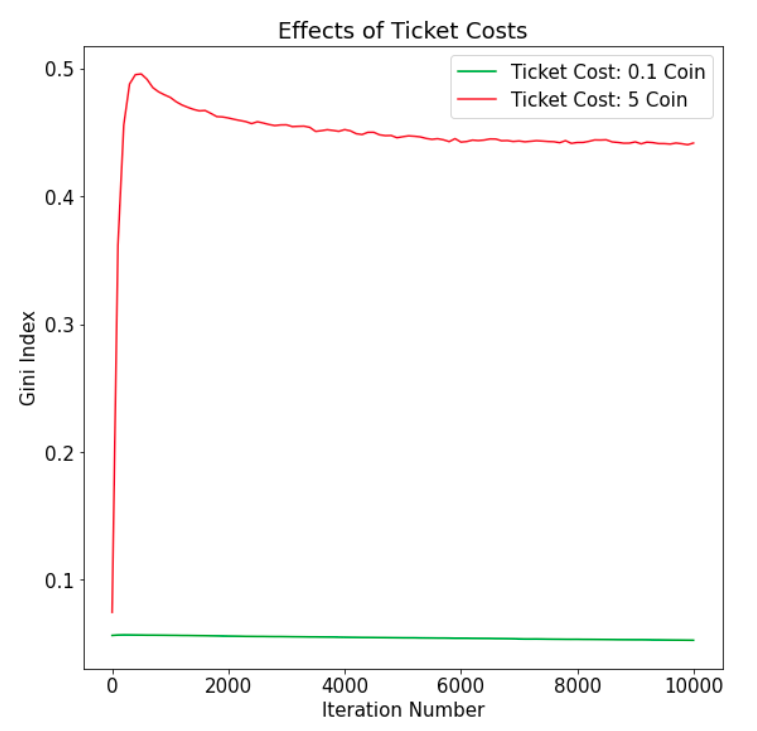
\includegraphics[width=0.5\textwidth]{03_Graphics/high_v_low}
\caption{Performance of Low vs. High Ticket Costs}
\end{center}
\end{figure}
Through the simulation of the Raffle Proof-of-Stake we designed, it was observed that in a network of 10,000 nodes beginning with a normal wealth distribution, the variable with the greatest impact on Gini coefficient was the participation cost or the cost per raffle ticket. With relatively lower ticket costs (i.e. 0.1 coin per ticket), the system performed very well with a miniscule change in Gini coefficient.

On the other hand, with high ticket costs (i.e. 5 coins per ticket), the system performed significantly worse, with the Gini coefficient rising at a much faster rate. Intuitively, this is due to the fact that increasing the ticket costs will also increase the size of the prize pool. This causes the shift in wealth to be in much larger increments after every raffle. Moreover, this theory is also supported by our findings during the investigation. We observed that with higher ticket costs, the average greed factor was higher than when the ticket costs were lower. This is because as the prize pool increased, so did the desire for nodes to participate. Therefore, an increase in ticket prices and the amount of participants caused the size of the prize pool to increase.

The same logic follows for low ticket costs. When ticket cost is 0.1 coin, the total prize pool decreases and the average node greed is also lower. We also realized that as more iterations passed, and new coins were mined, the reward from the raffle began to lose impact, and the effect on the Gini coefficient began to decrease. This is due to the average wealth of the network steadily increasing over iterations. So when the raffle ticket cost remained static, over time we observed the same effects as when ticket prices are very low. Therefore, we want to dynamically determine the cost of raffle tickets in accordance to the total wealth of the network.

By running the simulation multiple times with different pricing adjustments, we realized that the raffle Proof-of-Stake protocol works optimally when the average greed of the nodes remains at 0.5 (remember that greed is a ratio from 0 to 1). This means that when the network's greed is centered at the middle (or each node is "averagely" greedy), the distribution of wealth sets a good balance. With this implementation of raffle prizes, we then ran the simulations and compared them against the performances of the other Proof-of-Stake protocols we investigated. We observed that in terms of change in Gini coefficient, the raffle Proof-of-Stake performed the best.

From a network starting from a normal distribution of wealth, the increase in Gini coefficient was one one of the lowest compared to the other protocols (see Figure \textbf{\ref{fig:comp}}). In an already very centralized network, raffle Proof-of-Stake saw a very significant decrease in the Gini coefficient of the nodes. With these results, we can conclude that, on paper, raffle Proof-of-Stake outperforms all the other protocols we investigated in terms of reigning in the rate of increasing wealth centralization. In fact, if a network is already facing wealth centralization, the raffle Proof-of-Stake helps to mitigate it and redistribute the networks' wealth.
